\section{Amortized Cost}

\vspace{\parskip}

\begin{definition}[Amortized Cost] \index{amortized cost}
    The amortized cost per operation for a sequence of $n$ operations is the total cost of the operations divided by $n$.
\end{definition}

Generally, there are three methods for performing amortized analysis. Although all methods should give us the same answer, depending on the circumstances, some methods will be easier than others.

\begin{itemize}
    \item Aggregate analysis determines the upper bound $T(n)$ on the total cost of a sequence of $n$
    operations, then calculates the amortized cost to be $T(n) / n$.
    \item The accounting method determines the individual cost of each operation, combining its immediate execution time and its influence on the running time of future operations. We use the analogy of a bank account. Prior operations that may impact future operations can store some credits in the bank for uses by future operations. Usually, many short-running operations accumulate credits in small increments, while rare long-running operations use the credits.
    \item The potential method is like the accounting method, but the balance of the imaginary bank account at each state is given by the potential function.
\end{itemize}

As a starter, we will consider the data structure known as dynamic array. It is similar to a regular array, but its length changes according to the ``fullness'' of the array.

\index{dynamic array}

The array will be initialized with a fixed length. Upon calling \textsc{Insert}, it will insert an element into the array, and whenver the current array becomes full, we create a longer array and copy everything into the new array. Similarly, after calling \textsc{Delete}, we will shrink the array whenever the array becomes too empty. If we only consider the worst case, the runtime complexities are bad: $O(n)$ for both operations. However, if we look at the amortized cost, the runtime is actually smaller.

\begin{figure}[htbp]
    \captionsetup{singlelinecheck=false, font=footnotesize, labelsep=space, margin={0pt,1cm}, justification=raggedright}
    \includegraphics[width=0.4\linewidth]{figures/dynamic_arr_append.pdf}

    \hfill

    \caption[width=0.5\linewidth]{The dynamic array after the operation \textsc{Insert}(9). The length of the new array is doubled, and old elements are copied to the new array.}
\end{figure}

\section{Aggregate Method}

\section{Accounting Method}

\begin{figure}[htbp]
    \centering
    \includegraphics[width=0.6\linewidth]{figures/accounting_method_insert.pdf}
    \caption{<caption>}
\end{figure}

\section{Potential Method}

\vspace{\parskip}

\begin{definition}[Potential Function] \index{potential function}
    Let $D$ be some data structure with initial state $D_0$. For each $i = 1,2,\cdots,n$, let $c_i$ be the actual cost of the $i$-th operation and $D_i$ be the resulting data structure after applying the $i$-th operation to data structure $D_{i-1}$.

    The potential function $\Phi$ maps each data structure at state $i$, denoted $D_i$, to a real number $\Phi(D_i)$, which is the potential associated with data structure $D_i$.

    The amortized cost $\hat{c_i}$ of the $i$-th operation with respect to the potential function $\Phi$ is
    $$
    \hat{c_i} = c_i + \Phi(D_i) - \Phi(D_{i-1})
    $$
    And the total amortized cost of $n$ operations is
    $$
    \sum_{i=1}^{n} \hat{c_i} = \sum_{i=1}^{n} \left( c_i + \Phi(D_i) - \Phi(D_{i-1}) \right) = \sum_{i=1}^{n} c_i + \Phi(D_n) - \Phi(D_0)
    $$
\end{definition}